\documentclass[border=10pt]{standalone}

% \usepackage{pgfpages}
\usepackage{tikz}
\usetikzlibrary{shapes.misc, positioning,
 shadings, calc, arrows.meta}

\definecolor{lila}{rgb}{0.8, 0.8, 1}
\definecolor{myred}{rgb}{1, 0.5, 0.5}

\newcommand\wa{35mm}
\newcommand\ha{10mm}
\newcommand\rc{0.15cm}

\newcommand\wb{60mm}
\newcommand\hb{10mm}

\begin{document}

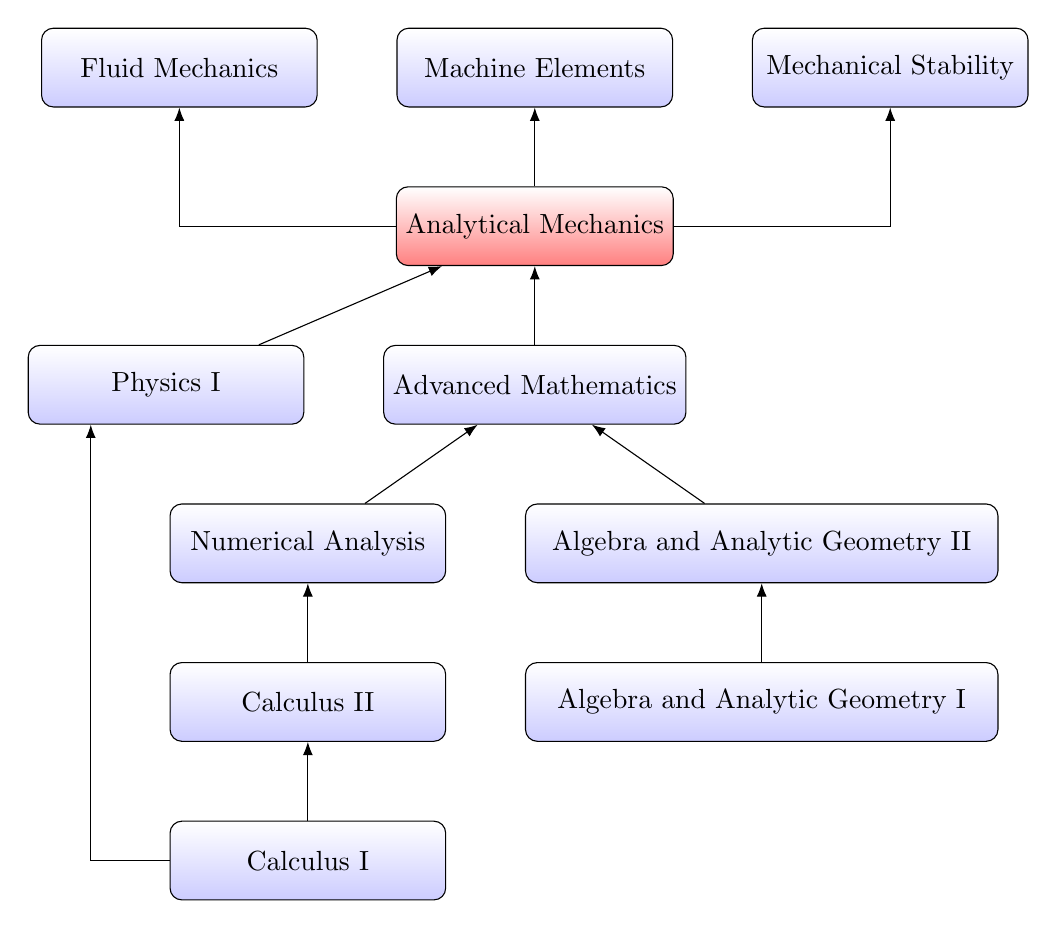
\begin{tikzpicture}[scale=1, every node/.style={scale=1}]
    % \draw[green,<-,line width=1pt] (7.5,0.7) -- (10,-0.2);
    % \draw [red, -latex] (0,0) to [out=70,in=180] (1,1) node[right, red] {Overfitting!};
    % \draw[rounded corners] (0, 0.5) rectangle (4, 1.5) {};

    \node (1) [draw, bottom color=lila, top color=white, rounded corners=\rc, minimum height=\ha, minimum width=\wa] {Calculus I};
    \node (2) [draw, bottom color=lila, top color=white, rounded corners=\rc, minimum height=\ha, minimum width=\wa, above=of 1] {Calculus II};
    \node (x) [draw, bottom color=lila, top color=white, rounded corners=\rc, minimum height=\ha, minimum width=\wa, above=of 2] {Numerical Analysis};

    \node (4) [draw, bottom color=lila, top color=white, rounded corners=\rc, minimum height=\ha, minimum width=\wb, right=of 2] {Algebra and Analytic Geometry I};
    \node (y) [draw, bottom color=lila, top color=white, rounded corners=\rc, minimum height=\ha, minimum width=\wb, right=of x] {Algebra and Analytic Geometry II};

    \node (6) [draw, bottom color=lila, top color=white, rounded corners=\rc, minimum height=\ha, minimum width=\wa, above=of $(x.north)!0.5!(y.north)$] {Advanced Mathematics};

    \draw[-Latex] (1) to (2);
    \draw[-Latex] (2) to (x);
    \draw[-Latex] (4) to (y);
    \draw[-Latex] (x) to (6);
    \draw[-Latex] (y) to (6);

    \node[coordinate] (w) [left=of 1] {};
    \node (7) [draw, bottom color=lila, top color=white, rounded corners=\rc, minimum height=\ha, minimum width=\wa, left=of 6] {Physics I};
    \draw[-Latex] (1) -- (w) -- (w|-7.south);

    \node (M) [draw, bottom color=myred, top color=white, rounded corners=\rc, minimum height=\ha, minimum width=\wa, above=of 6] {Analytical Mechanics};
    \node (8) [draw, bottom color=lila, top color=white, rounded corners=\rc, minimum height=\ha, minimum width=\wa, above=of M] {Machine Elements};
    \node (9) [draw, bottom color=lila, top color=white, rounded corners=\rc, minimum height=\ha, minimum width=\wa, right=of 8] {Mechanical Stability};
    \node (10) [draw, bottom color=lila, top color=white, rounded corners=\rc, minimum height=\ha, minimum width=\wa, left=of 8] {Fluid Mechanics};

    \draw[-Latex] (7) to (M);
    \draw[-Latex] (6) to (M);
    \draw[-Latex] (M) -| (9);
    \draw[-Latex] (M) -| (10);
    \draw[-Latex] (M) -- (8);

\end{tikzpicture}


\end{document}
